\begin{figure}
\centering
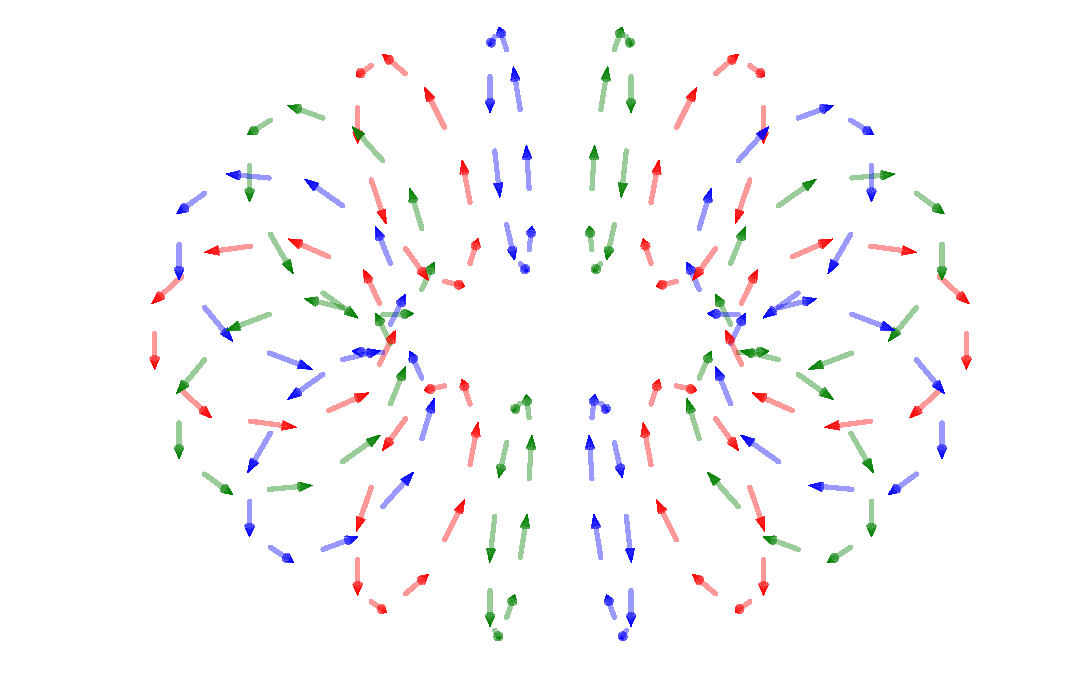
\includegraphics[width=0.8\textwidth]{papers/wirbelringe/fig/wirbelring_RGB.pdf}
\caption{Typischer idealer Wirbelring. 
Dargestellt durch momentane Bewegungsvektoren unterschiedlicher Teilchen in regelmässigen Abstand. 
Zur besseren Übersicht sind Teilchen eines Wirbels mit derselben Farbe markiert. 
Unterschiedliche, benachbarte Wirbel haben unterschiedliche Farben. \label{Wirbelringe:fig:generell}}
\end{figure}